%\documentclass{article}
%\usepackage{graphicx}

%\title{Data Analysis}
%\begin{document}
\section{Initial Results}
Since the distance traveled is calculated in tenths of a degree, the computer used was not powerful enough to plot
a full year in any reasonable amount of time. The best that could be done was a period of ten days. Since the velocity
takes units of meters per second, time was fed in in intervals of 86400 seconds. The resulting graph of the distance
between Earth and Mars, Figure (\ref{DiffPlot}), was unreasonable. Since Earth is closer to the sun, its average radius
will be lower. According to the velocity equation given in the last section, this means the average velocity of Earth 
should be considerably higher than that of Mars. Thus, Earth should make a full orbit before returning to close
proximity with Mars. This should put the time period of the Earth-Mars distance on the scale of about a year.
However, figure (\ref{DiffPlot}) shows an orbital period of about 15 Days. This could have been due to Earth's speed 
being calculated too high but figure(2) shows that both planets take a maximum velocity at their 
semimajor axis, and a minumum 180 degrees after. This is to be expected from equations of the form $a(1+cos(\theta))$ where a is a constant. 
%I realize that typing Figure(2) is unprofessional but no matter how many times I typed the reference it still put 
%figure(1) for some odd reason
\begin{figure}
	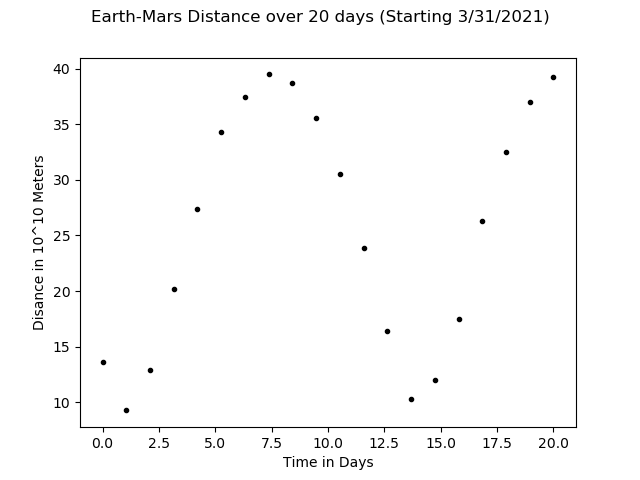
\includegraphics[scale = 0.8]{DistancePlot.png}
	\label{DiffPlot}
	\caption{Distance between Earth and Mars over time as determined by the equations from Section 1.1.1}
\end{figure}

\begin{figure}
	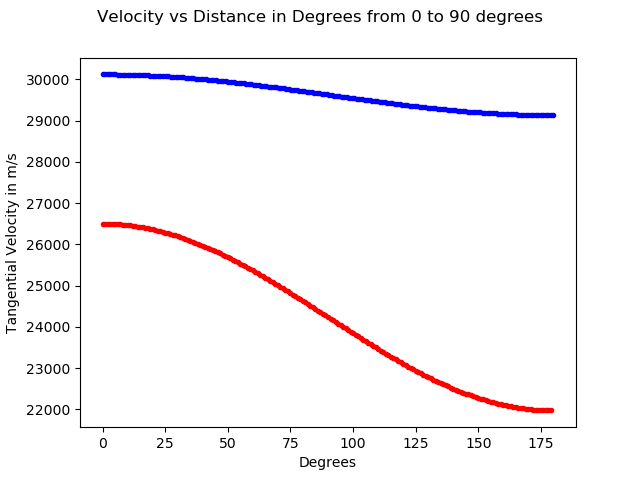
\includegraphics[scale = 0.8]{VelocityPlot.png}
	\label{VelocityPlt}
	\caption{Velocity of Earth and Mars over 180 degrees of rotation}
\end{figure}

\section{Trouble Shooting}
The issue appeared to be the width of the $\Delta\theta$ intervals, as a larger interval will result in a decreasingly
accurate velocity - this is expanded on in section \ref{VelErrSec}. To test this, another plot was generated with $\Delta\theta$ = 1 degree rather than 1 tenth of a degree. Were this the cause for the smaller distance period, the new
figure would have a noticably smaller orbital period. However, the new plot (figure (\ref{DiffPlot2})), while less 
accurate, has roughly the same distance period. All of the constants used in the program were double and triple 
checked, but the source of this strangely small distance period is still unclear.
\begin{figure}
	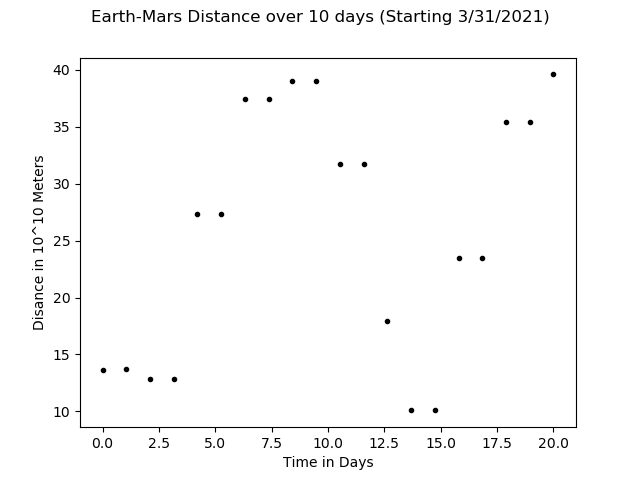
\includegraphics[scale = 0.8]{DistancePlot2.png}
	\label{DiffPlot2}
	\caption{Plot of Difference over time where the $\Delta\theta$ = 1 degree}
\end{figure}
\section{Visualizing Velocity Error}
\label{VelErrSec}
It is helpful to visualize the error in the approximation of constant velocities over small intervals of $\Delta\theta$.
In order to get an idea of the error of assuming these constant velocities, it is helpful compare the starting velocity
of an interval (the one used) to the velocity half way through that interval. This error is shown in equation \ref{Error},
where $v_{1}$ is the velocity at one tenth of the corresponding value on the x-axis and $v_{2}$ 
is the velocity 0.05 degrees later. Figure(\ref{ErrPlot}) shows that the error peaks out at 90 degrees and never exceeds
.0014\%. While this would seem to indicate that the method is reliable, the final results make this doubtful.
\begin{equation}
	Error = \frac{|v_{2}-v_{1}|}{v_{2}}100
	\label{Error}
\end{equation}
\begin{figure}
	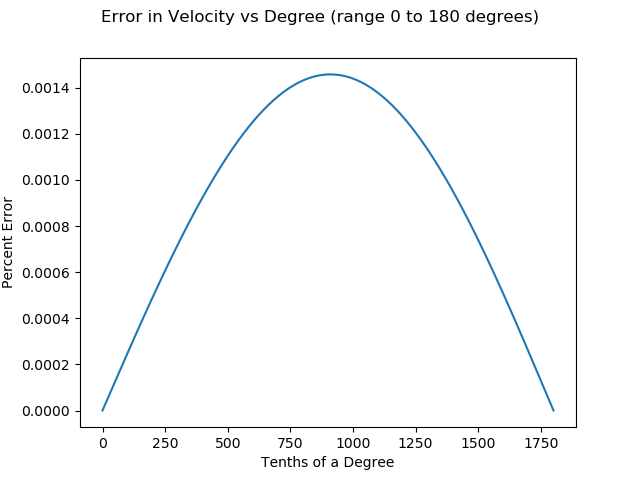
\includegraphics[scale = 0.8]{VelocityError.png}
	\label{ErrPlot}
	\caption{Error based on variation of velocity between two tenths of a degree}
\end{figure}
%\end{document}
